\documentclass[12pt, letterpaper]{article}
\usepackage[utf8]{inputenc}

%Russian-specific packages
%--------------------------------------
\usepackage[T2A]{fontenc}
\usepackage[utf8]{inputenc}
\usepackage[ukrainian]{babel}
%--------------------------------------

\usepackage[margin=0.5in]{geometry}

\title{AI}
\author{argoniton}
\date{March 2017}

\usepackage{natbib}
\usepackage{graphicx}

% http://www.auburn.edu/~tamtiny/Symbols.pdf



\begin{document}

\maketitle

\begin{figure}[h!]
\centering
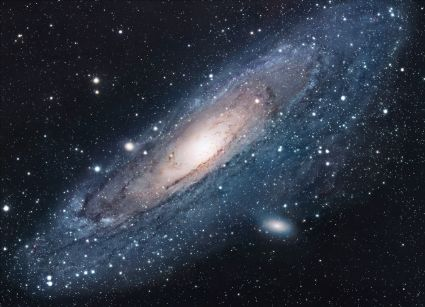
\includegraphics[scale=1.7]{universe.jpg}
\caption{The Universe}
\label{fig:univerise}
\end{figure}

Створв винайшов розробив
З'явився
Перші ідеї розумних машин вперше з'явилися в грецькій міфології
Після вв2 вже стало можливим створювати програми, що виконували сладні завдання

\section{Technical}

Створв винайшов розробив
З'явився
Перші ідеї розумних машин вперше з'явилися в грецькій міфології
Після вв2 вже стало можливим створювати програми, що виконували сладні завдання

\section{Антична історія}
Грецькі міфи про Хефаєса, хто створив механічного офіціанта.
І про Талоса, хто створив ідею розумних роботів.
Інші міфи античності включають людиноподібні артифакти.
Багато механічних іграшок створені  Archytas of Tarentum, Hero, Daedalus та інш.
4СТ. ДО Н.Е.
Арістотель винайшов силогістичну логіку.
Це перша формальна дедуктивна міркуюча система.
\subsection{Пізня Античність}
13СТ
Філосови Roger Bacon та Albert the Great, сказали винайшли Говорячі Голови
Ramon Lull винайшов машину для знаходження істиннит тверджень з комбінацій
Al-Jazari розробив першого програмованого музикального робота
\section{Середньовіччя}
15СТ
Винайдення притнера - рухомий друк. Gutenberg Bible printed (1456)
\section{Відродження}
15-16СТ
Створено годинник.

16СТ
Clockmakers розширили своє ремесло до створення механічних звірів.
Наприклад DaVinci's walking lion (1515).
Rabbi Loew of Prague створив Golem, a clay man brought to life (1580).
\section{Просвітництво}
17СТ
На початку ст. Descartes ствердив, що звірі це лише складні механічні створіння
Багато інших філософів запропонували свої варіації та вдосконалення цієї ідеї
Pascal сконструював першу механічну обчислювальну машину 1642
Thomas Hobbes опублікував The Leviathan (1651)
Це перша математична та комбінаторна теорія мислення
Арифметична механіка розроблена Sir Samuel Morland 1666
Лейбніц покращив машину Паскаля щоб множити та ділити - Step Reckoner (1673)
Передбачив універсальне числення мислення, де аргументи визначаються механічно

18СТ
Різноманітні механічні іграшки, качка, що грає в шахи The Turk (1769).
Edgar Allen Poe  сказав, це не машина, інакше вона вигравала б. 1836

19СТ
Joseph-Marie Jacquard винайшов Jacquard loom, перша програмована машина
Вона отримувала інструкції з пробитих карт
The Luddites 1811-1816 рух, ідея якого руйнування машин
Mary Shelley опублікував історію про Frankenstein's monster (1818
Charles Babbage & Ada Byron сконструювали програмований математичний калькулятор
Робоча модель Analytical Engine (1832) була побудована 2002
George Boole розробив бінарну алгебру, модель "законів мислення" у 1854
Сучасна логіка висловлювань Gottlob Frege у Begriffsschrift 1879 
Вона була покращена та вдосконалена Russell,Tarski, Godel, Church та інш

20СТ перша половина
Bertrand Russell та Alfred North Whitehead опублікували Principia Mathematica
Це була революція формальної логіки.
Russell, Ludwig Wittgenstein, and Rudolf Carnap логічний аналіз знання
Torres y Quevedo створив "шахматну" машину 'Ajedrecista' перша компютерна гра
Karel Capek's гра "R.U.R." 1921 (London opening, 1923) з'явилося слово робот
Alan Turing запропонував the universal Turing machine (1936-37)
Electro електрична людина від Westinghouse Electricat, Sparko електрична собака.
Warren McCulloch & Walter Pitts логічне числення - основа нейромереж
Arturo Rosenblueth, Norbert Wiener & Julian Bigelow слово  "cybernetics" 1943
Книга Wiener's названа цим ім'ям 1948
Emil Post довів що production system - загальний обчилювальний механізм 1943
 Post also did important work on completeness, inconsistency, and proof theory.
George Polya книга про thinking heuristically названа How to Solve It у 1945
Vannevar Bush опублікував As We May Think передбачення, що машини служать людям
Grey Walter ексерементує з автономними роботами  Elsie and Elmer 1948-9
Його припущення що мала кількість мозкових клітин забезпечує складну поведінку
A.M. Turing публікує "Computing Machinery and Intelligence" (1950) Тест тюрінга
Claude Shannon аналіз гри в шахи Programming a computer to play chess" (1950)
Isaac Asimov публікує three laws of robotics (1950).

Modern History
Сучасна історія штучного інтелекту починається з розвитком компютерів.
1956
McCarthy створив термін "штучний інтелект"
перша програма Logic Theorist (LT)
1957
General Problem Solver (GPS) Newell, Shaw & Simon
1952-62
Перша гра Arthur Samuel checkers
1958
John McCarthy винайшов Lisp language
Herb Gelernter & Nathan Rochester (IBM) described a theorem prover in geometry
John McCarthy's Programs with Common Sense
Late 50's & Early 60's
Margaret Masterman (Cambridge) design semantic nets for machine translation
1961
James Slagle  the first symbolic integration program SAINT
1962
First industrial robot company, Unimation, founded.
1963
computers can solve the same analogy problems as are given on IQ tests.
Sketchpad introduced the idea of interactive graphics into computing
Computers and Thought, the first collection of articles about artificial intelligence.
1964
Danny Bobrowshows that computers can understand natural language
Bert Raphael SIR programrepresentation of knowledge for question-answering systems
1965
J. Alan Robinson invented a mechanical proof procedure, the Resolution Method
Joseph Weizenbaum (MIT) built ELIZA
1966
Ross Quillian demonstrated semantic nets.
First Machine Intelligence workshop at Edinburgh 
Negative report on machine translation
1967
Dendral program хімія First successful knowledge-based program for scientific reasoning.
Joel Moses demonstrated the power of reasoning. First knowledg program in mathematics.
Richard Greenblatt at MIT built a knowledge-based chess-playing program
Late 60s
Doug Engelbart invented the mouse at SRI.
1968
Marvin Minsky, demonstrating limits of simple neural nets.
1969
SRI robot, Shakey, demonstrated combining locomotion, perception and problem solving.
Roger Schank (Stanford) defined conceptual dependency model for natural language 
Robert Wilensky and Wendy Lehnert, for use in understanding memory by Janet Kolodner.
First International Joint Conference on Artificial Intelligence held in D.C.
1970
SCHOLAR- interactive program for computer-aided instruction based on semantic nets
Bill Woods described Augmented Transition Networks language understandin'
Patrick Winston's PhD program, ARCH, world of children's blocks.
Early 70's
Jane Robinson & Don Walker influential Natural Language Processing group
1971
Terry Winograd thesis computers can understand English sentences in a WOCB SHRDLU
1972
Prolog developed by Alain Colmerauer.
1973
The Assembly Robotics group at Edinburgh University builds Freddy
1974
Ted Shortliffe rule-based systems for knowledge in medical domain
Earl Sacerdoti developed one of the first planning programs, ABSTRIPS
1975
Marvin Minsky published his widely-read and influential article on FRAMES
The Meta-Dendral learning program produced new results in chemistry
Mid 70's
Barbara Grosz focus of discourse and anaphoric references in NLP
Alan Kay  Smalltalk language object-oriented programming
David Marr and MIT colleagues describe the "primal sketch" and visual perception.
1976
Doug Lenat demonstrated the discovery model search for interesting conjectures.
Randall Davis demonstrated the power of meta-level reasoning
late 70's
Stanford's SUMEX-AIM resource,demonstrates the power of the ARPAnet
1978
Version Spaces for describing the search space of a concept formation program.
Nobel Prize in Economics for his theory of bounded rationality,
The MOLGEN program  object-oriented representation of knowledge -> gene-cloning
1979
Mycin MYCIN's representation of knowledge style of reasoning
CHI system for automatic programming.
Drew McDermott non-monotonic logics and formal aspects of truth maintenance.
1980's
Lisp Machines developed and marketed.
First expert system shells and commercial applications.
1980
HEARSAY-II speech understanding system
American Association of Artificial Intelligence (AAAI) 
1881
Danny Hillis - connection machine, a massively parallel architecture power to AI
1983
Interval Calculus, the first widely used formalization of temporal events.
Mid 80's
Neural Networks become widely used with the Backpropagation algorithm
1985
The autonomous drawing program, Aaron, created by Harold Cohen
1987
Marvin Minsky The Society of Mind, a description of the mind as many agents.
1989
Dean Pomerleau (An Autonomous Land Vehicle in a Neural Network)
1990's
#machine learning, intelligent tutoring, case-based reasoning, multi-agent planning, scheduling, uncertain reasoning, data mining, natural language understanding and translation, vision, virtual reality, games, and other topics.
Rod Brooks humanoid robot
TD-Gammon learning
EQP theorem prover at Argonne National Labs proves the Robbins Conjecture
The Deep Blue chess program beats the current world chess champion, 
NASA’s pathfinder mission made a successful landing surface of Mars. 
Web crawlers and other AI-based information extraction programs
Demonstration of an Intelligent Room and Emotional Agents at MIT's AI Lab
2000's
Interactive robot pets (a.k.a. "smart toys") become commercially available,
Cynthia Breazeal KISMET, a robot with emotions.
Stanford's autonomous vehicle, Stanley, wins DARPA Grand Challenge race.
The Nomad robot explores remote regions of Antarctica 
https://aitopics.org/i2kweb/aitopics/misc/brief-history

''I always thought something was fundamentally wrong with the universe'' \citep{Kimbark197109}
\section{Conclusion}
''I always thought something was fundamentally wrong with the universe'' \citep{adams1995hitchhiker}

\bibliographystyle{plain}
\bibliography{references}


\end{document}
